\chapter{Introduction}
\label{ch:Introduction}

\stress{\textbf{Disclaimer to this document:} This is a template with some additional thesis information and a sample structure. The structure includes the chapters most commonly needed in a thesis. Neither the order nor the chapter titles are fixed and will most likely have to be adapted to your specific thesis. However, the notes here should help you to get an idea what each chapter could be about and how to use this template. When in doubt, please talk to your supervisor(s).} \\

Your thesis should start with an introduction. The introduction is supposed to motivate your thesis.
Discuss the relevance of your topic, why are you looking into it, why is it relevant in the field? Cite important research related to your motivation.
Briefly state the problem as in the abstract and repeat the contribution, for example in the form of research questions. 

Give an outline of your thesis.

Testing the glossaries package \gls{rmse}


Below, you will find an example figure (\Cref{fig:example}). Please use the caption of your figures to describe everything in the figure, additionally to what you have written about the figure in the text. Everyone should be able to understand the figure just reading its caption.

\begin{figure}[h!]%
\centering
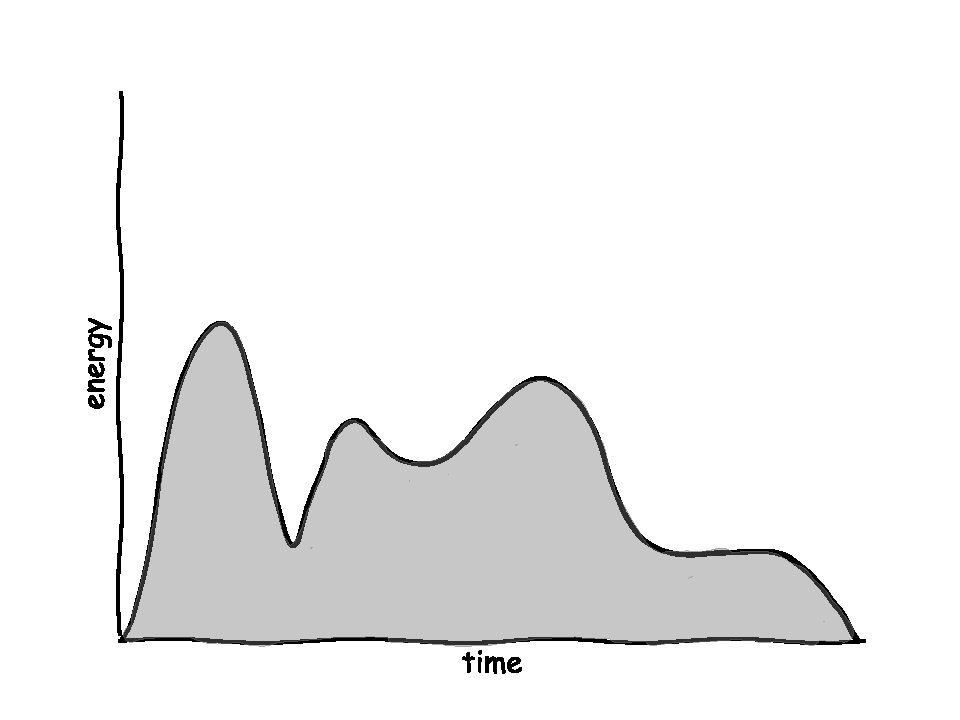
\includegraphics[width=0.5\columnwidth]{plots/Figure_2_demand}%
\caption{This is an example figure. It shows a fictional demand of energy (in grey) over time.}%
\label{fig:example}%
\end{figure}
